\chapter{Graph Mining}
\textit{Graphs} are used in a variety of domains - chemical compounds, protein structures, traffic flow, program control flow, and so on. Modeling data with graphs gives enormous flexibility to the modeler for storing the elements, elements' attributes, relationship between two elements, relation between a set of elements, type of relation, and so on.

\textbf{Graph Mining} is essentially the problem of discovering repetitive interesting patterns/sub-graphs occurring in the input graphs. Standard data mining algorithms are based on the \textit{flat transaction representation} (sets of items). Datasets with structures, layers, hierarchy and/or geometry often do not fit well in this flat transaction setting. A social network is one such dataset. 

Some of the major tasks in graph mining are node classification, link prediction, and clustering. Traditional machine learning techniques cannot be applied directly on graphs because of the non-euclidean nature of the data structure. Analyzing graphs with machine learning has garnered a lot of interest recently, given the expressive power of graphs.

\section{Convolutional Neural Networks}

\textit{Convolutional Neural Network (CNN)} is a deep learning architecture inspired by the natural visual perception mechanism of the living creatures. A convolution is the simple application of a filter to an input that results in an activation. Repeated application of the same filter to an input results in a map of activations called a feature map, indicating the locations and strength of a detected feature in an input, such as an image. It has the ability to automatically learn a large number of filters in parallel specific to a training dataset under the constraints of a specific predictive modeling problem, such as image classification. The keys of \textit{Convolutional Neural Networks (CNN)} are local connection, shared weights and the use of
multi-layer structure.

\section{Graph Neural Networks}

Graphs are locally connected structure. The shared weights reduce the computational cost compared with traditional spectral graph theory. The multi-layer structure is the key to deal with hierarchical patterns, which captures the features of various sizes. \textit{Graph Neural Networks (GNN)} are deep learning methods that operate on graphs. They have high interpretability and acceptance. The first motivation of GNNs roots in CNNs.  However, CNNs operate only on Euclidean data like images (2D) and text (1D). Also, there isn't a natural order of nodes in the graph. This requires a model to traverse all the possible orders of nodes, which is infeasible. To solve this problem, GNNs propagate on each node respectively, ignoring the
input order of nodes. In other words, the GNN output is invariant for the input order of nodes. 

The other motivation for GNNs comes from \textit{graph embedding}, which learns to represent graph nodes, edges or sub-graphs in low-dimensional vectors. Traditional direct embedding methods lack the ability to generalize, they cannot deal with dynamic graphs or generalize to new graphs.  The target of GNN is to learn a state embedding which contains the information of neighborhood for each node. Based on CNNs and graph embedding, GNNs are proposed to collectively aggregate information from social network graphs.

\begin{figure}
    \centering
    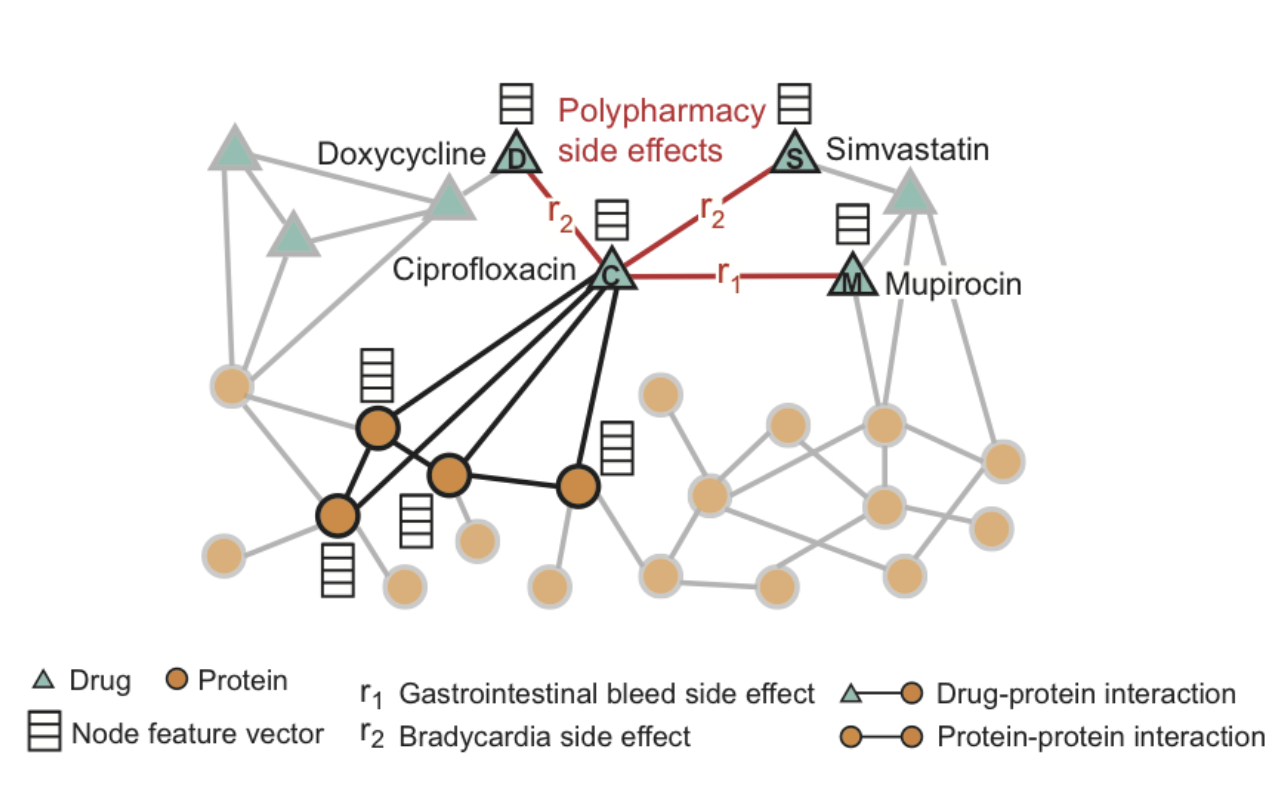
\includegraphics[height=6cm]{tex/img/drug-protein interaction.png}
    \caption{A model that predicts specific drug-drug interaction effects.}
    \label{fig:my_label}
\end{figure}
